\documentclass[unicode,11pt,a4paper,oneside,numbers=endperiod,openany]{scrartcl}

\usepackage{ifthen}
\usepackage[utf8]{inputenc}
\usepackage{graphics}
\usepackage{graphicx}
\usepackage{float}
\usepackage{hyperref}

\pagestyle{plain}
\voffset -5mm
\oddsidemargin  -2.5mm
\evensidemargin 0mm
\marginparwidth 2cm
\marginparsep 0pt
\topmargin 0mm
\headheight 0pt
\headsep 0pt
\topskip 0pt        
\textheight 255mm
\textwidth 165mm

\newcommand{\duedate} {}
\newcommand{\setduedate}[1]{%
\renewcommand\duedate {#1}}
\newcommand\isassignment {false}
\newcommand{\setassignment}{\renewcommand\isassignment {true}}
\newcommand{\ifassignment}[1]{\ifthenelse{\boolean{\isassignment}}{#1}{}}
\newcommand{\ifnotassignment}[1]{\ifthenelse{\boolean{\isassignment}}{}{#1}}

\newcommand\serieheader[6]{
\thispagestyle{empty}%
\begin{flushleft}
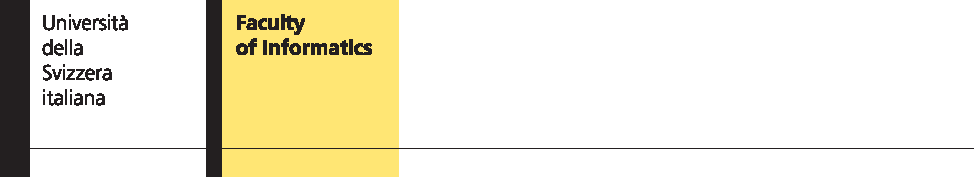
\includegraphics[width=\textwidth]{./assets/logo-info.pdf}
\end{flushleft}
  {\large\ignorespaces #3 \hspace{\fill}\ignorespaces #4}\\
  \noindent%
  \bigskip
  \hrule\par\bigskip\noindent%
  \bigskip {\ignorespaces {\Large{\textbf{#5}}}
  \hspace{\fill}\ignorespaces \large \ifthenelse{\boolean{\isassignment}}{\duedate}{#6}}
  \hrule\par\bigskip\noindent%  \linebreak
 }

\makeatletter
\def\enumerateMod{\ifnum \@enumdepth >3 \@toodeep\else
      \advance\@enumdepth \@ne
      \edef\@enumctr{enum\romannumeral\the\@enumdepth}\list
      {\csname label\@enumctr\endcsname}{\usecounter
        {\@enumctr}%%%? the following differs from "enumerate"
	\topsep0pt%
	\partopsep0pt%
	\itemsep0pt%
	\def\makelabel##1{\hss\llap{##1}}}\fi}
\let\endenumerateMod =\endlist
\makeatother

\usepackage{textcomp}


\begin{document}

\graphicspath{ {./assets/} }

\setassignment
\setduedate{Final Report}

\serieheader{Artificial Intelligence}{2021}{Student: Edoardo Riggio}{}{AI Cup 2021}{}
\newline

\tableofcontents

\newpage

\section{Abstract}
The purpose of this competition was to find the shortest possible tours given a number of Euclidean TSP problems. In order to do so, we had to propose, implement and test one or more heuristic algorithms learned during the semester.

\section{Algorithms}
I've decided to implement the \textit{Best Nearest Neighbors} heuristic algorithm and the \textit{2.5-opt} optimizer.

\subsection{Best Nearest Neighbors}
This algorithm is divided in two parts, the first is the loop on the $n$ nodes of the graph, and the second is the actual computation of the path. \\ \\
In the first part, every point of the graph is considered as the starting point of a new path. The path with the shortest length is the one chosen as the solution of the \textit{Best Nearest Neighbors} algorithm. In the second part of the algorithm, the starting node is taken from the first part, and the path is actually computed. The computation starts from the starting node and continues by selecting the nodes that have the shortest Euclidean distance between one another. \\ \\
Since the running time of this algorithm is relatively high for problems such as \textit{fl1577}, I've decided to use the flag \verb|-O3| when compiling the code. This made the code run much faster while still keeping the same results.

\subsection{2.5-opt}
This algorithm is an extension of the 2-opt algorithm. In this case we consider the gain of a 2-opt swap, as well as two node shifts -- which are 3-opt moves. By finding out which of these moves is the best -- i.e. returns the shortest path -- the swap is performed. \\ \\
This algorithm is ran for every single pair of points in the graph and until no further improvement is possible.

\section{Results}
The combination of the two algorithms described above made me reach an average gap of $4.1\%$ between the best possible solution and my solution. \\ \\
As per requirements, the results are available in the \verb|.xls| file given that was given to us. Alternatively, it is also available in the \verb|README| file of this repository.

\section{Technical Details}
In order to write my submission for the AI cup I've used C++. In my solution I've implemented a class that reads and stores the problem, and one that stores the solvers for the problem. The actual solvers -- i.e. the \textit{Best Nearest Neighbors} algorithm and the \textit{2.5-opt} algorithm -- are implemented as functions that are passed to the solver class. A full documentation of both classes and functions can be found either as an \verb|html| page or as a \verb|pdf| file inside of the docs directory. \\ \\
In order to run the solvers, just type:

\begin{verbatim}
    make run
\end{verbatim}
Inside of the root directory of the repository. This will compile and run the binary, making no further action necessary. The results of the solvers are displayed in a similar fashion as we saw in class during the tutorials.

\end{document}























